% Chapter Template

\chapter{Visualising real-world networks} % Main chapter title

\label{Chapter6} % Change X to a consecutive number; for referencing this chapter elsewhere, use \ref{ChapterX}


In the previous chapter, tools were developed to allow for simple logs and diagrams to be generated from the log files produced by the test frameworks.
This chapter will continue answering the fourth research question "\fourthRQ" by implementing the functionality to use these tools to analyse real-world Serval networks.
This chapter will also outline the methodology for comparing real-world and emulated tests to determine the simulation fidelity of the test framework.

\section{Generating diagrams of the real-world}   
To begin to analyse the differences between the emulated Serval networks and those of real-world networks, identical Serval networks need to be run in both emulation using the test framework and in the real world.
By using the tools created throughout this thesis, the differences and similarities in the functionality of the networks can be analysed.
To do this however, some changes will need to be made to the program to support the generation of real-world Serval tests.
The first of these is that initial log files will need to be made for the real-world tests.
This log file is simply a single compiled file of the logs in the real-world tests that the program will use as the input to generate the simple log file and the diagrams.

Further, some changes are required to be made to the tool.
These changes required include moving to using just LBARD for the generation of radio major events since real-world tests don't use Fakeradio, and retrieve node SIDs from Servald since the test framework can not be used for determining the SIDs.

If solutions to these changes are found that exist solely within Servald or LBARD, then these solutions will be applicable to analysis of both the emulated test framework and real-world tests.

\subsection{Creating initial log file}
To create the initial log file to be used for real-world tests, multiple log files will need to be manually combined to create the single initial log file that the program requires.
This log file will simply contain all the log outputs from the Servald and LBARD processes that are involved in the real-world test.

This log file needs to follow the same format as that of the log files:
\begin{itemize}
    \item Four lines detailing the name, result, and start and finish time for the test
    \item Each LBARD process with a line proceeding each process listing which LBARD process it is
    \item Each Servald process with a proceeding line detailing which Servald process it is
\end{itemize} 

Additionally, the SIDs for each of the nodes will need to be listed at the top of the file. 
This is because as the initial log file is processed, any references to a SID involve a lookup to determine which node this is referring to, requiring these SIDs to be listed at the beginning of the file to remove the need to preprocess this file.
For emulated tests this was not necessary, as these SIDs are reported by the test framework at the beginning of the log file.
A combined real-world log file may look similar to \figurename{ \ref{fig:chapter6RealWorldLog}}.

\begin{figure}
    \begin{centering}
\begin{lstlisting}[basicstyle=\small, breaklines, frame=single]
Name:     FieldTest
Result:   PASS
Started:  2020-08-24 13:22:55.044
Finished: 2020-08-24 13:23:32.497
++++++++++ fork[1] %lbardA log.stdout ++++++++++
469:My SID as hex is [SID]
++++++++++ fork[1] %lbardB log.stdout ++++++++++
469:My SID as hex is [SID]
++++++++++ fork[1] %lbardA log.stdout ++++++++++
[LBARD log file for node A]
++++++++++ fork[1] %lbardB log.stdout ++++++++++
[LBARD log file for node B]
#----- var/servald/instance/A/servald.log -----
[Servald log file for node A]
#----- var/servald/instance/B/servald.log -----
[Servald log file for node B]
\end{lstlisting}
        \caption{Example format of a compiled real-world log file with two nodes, A and B}
        \label{fig:chapter6RealWorldLog}
    \end{centering}
\end{figure}

Additionally, to ensure that real-world tests are producing the appropriate log output to create network diagram, every field test must have some specific configuration enabled at a minimum.
For LBARD processes, the flags that must be set are:
\begin{lstlisting}
    bundles
    pieces
    announce
    message_pieces
    sync
    sync_keys
    \end{lstlisting}

With these flags, LBARD will produce the minimum log output required to generate diagrams. 

For \texttt{servald} processes no specific configurations are required, however it is recommended to run each process with the following configuration as a minimum:
\begin{lstlisting}
    set log.console.show_pid on 
    set log.console.show_time on 
    set debug.server on 
    set debug.mdprequests on 
    set debug.httpd on 
    set debug.rhizome_manifest on
    set debug.rhizome_sync_keys on
    set debug.msp on
    set debug.config on
    set debug.mdprequests on
    set debug.mdp_filter on
    set debug.verbose on
\end{lstlisting}
These configurations will allow for a good coverage of Servald functionality, and provide the necessary information for a deeper analysis of real-world tests.


\subsection{Adding support for real-world tests}
Once the initial log file has been created for the real-world test, this can then be processed by the tool.

While the tool will be able to produce a simple log file, the tool will fail to create proper PDF or ASCII outputs as it is only able to create major events from \texttt{servald} WiFi transfers.
This is due to the program's reliance on \texttt{fakeradio} for determining major events.
For test results produced by the test framework this was a reasonable assumption, as \texttt{fakeradio} handles all the radio traffic.
However, the real-world tests do not simulate radio connections, and as such a new way of determining radio major events must be implemented.

To achieve this, if the presence of \texttt{fakeradio} is not detected in the input log file, then every time LBARD announces that it sends a bundle piece, this is used as a major event.
An example of this log output can be seen in \figurename{ \ref{fig:chapter6RLBARDSent}}.

\begin{figure}
    \begin{centering}
\begin{lstlisting}[basicstyle=\small, breaklines]
    >>> [13:13.02.983 662D*] I just sent manifest piece [0,128) of [BID] for [receiving SID]
\end{lstlisting}
        \caption{LBARD output when sending a bundle piece}
        \label{fig:chapter6RLBARDSent}
    \end{centering}
\end{figure}

As LBARD will only report that it is sending a bundle to a single node in this log output, the assumption will need to be made that LBARD is sending this piece to all its neighbours.
Despite this, using the LBARD log output presents an improvement, as LBARD reports the start and end bytes of the bundle piece it is sending, allowing for the display of a bundle bitmap.
This allows for easier analysis of how LBARD is sending pieces through the network and will be described in the next section.

With these changes made, the compiled log files of the real world tests can then be run through the tool and all output types will function as expected.

\subsection{Displaying bundle bitmaps}
To assist with the analysis of LBARD sending and receiving bundles and bundle pieces, bundle bitmaps can be used to display the count of times that a specific section of a bundle body or manifest has been sent to a node.
This is useful when analysing LBARD networks, as a long-standing bug in LBARD revolves around bundles not being properly marked as received.
By analysing these bundle bitmaps, Serval testers will be able to determine what pieces of a bundle have been sent excessively or not at all.

\subsubsection{Calculating bitmap partitions}
The bitmap partitions refer to the start and end bytes that a node receives for this bundle.
To calculate the bitmap partitions, every time LBARD on a node reports that it sends a bundle piece, add the start and end byte values to an array for each of the destination nodes.
At the conclusion of the simple log processing, each node has an array of bitmap partitions for every bundle that was sent during the test over LBARD.

While this will produce an accurate view of the pieces that a node has been sent throughout the test, this does not provide an adequate level of granularity.
With the exception for the last piece, bundle pieces always have a granularity of 64 bytes \parencite{rhizomeDocumentation}, however LBARD often attempts to send pieces in 128 byte increments \parencite{rhizomeDocumentation}.
Thus, to account for this necessary level of granularity, the program must add any non-existent bundle partitions that are a multiple of 64 and less than the maximum byte value that this node has received.
To do this, the program iterates through the sorted array of byte partitions, and if any multiple of 64 is missing from where it should be in the array, appends it to the end.
After it iterates through the array, the program sorts the array, giving a complete bundle bitmap for both the body and manifest with a granularity of 64 bytes (except the last piece which may be less than 64 bytes).


\subsubsection{Displaying bitmaps}
Once the bitmap partitions had been calculated for every node, the bitmaps can then be displayed.
To display these bitmaps, both the partitions and a current count of the number of times that a piece has been sent that contained that partition must be calculated.
These bitmaps are displayed alongside each LBARD major event in both the ASCII and PDF outputs.
As these are related to a major event, this count must present a count at the time of the major event.

To display the current bitmap partition count during the ASCII or PDF output, every time a LBARD transfer major event is encountered throughout the displaying of this bitmap, each of the receiving nodes of this bundle transfer have their bitmap counts adjusted.
The tool uses the message type and the start and end bytes of this piece and increments the count of every partition for that bundle for each receiving node between the start and end bytes.
With this, a 'live' bitmap of each of the bundles can be displayed for each of the receiving nodes at the time of the major event.

An example of the bitmaps for the ASCII output can be seen in \figurename{ \ref{fig:chapter6ASCIIPartition}}.

\begin{figure}
    \begin{centering}
\begin{lstlisting}[basicstyle=\small, frame=single, breaklines]
57: [ 13:22:54.982] Sent body piece [0,50) of 5B59E446*
A -> BCD
  Manifest Bitmap (B):
  | [0,64)    | [64,128)  | [128,192) | [192,256) |
  | 1         | 1         | 1         | 1         |
  Body Bitmap (B):
  | [0,50)     |
  | 2          |
  
  Manifest Bitmap (C):
  | [0,64)    | [64,128)  | [128,192) | [192,256) |
  | 1         | 1         | 1         | 1         |
  Body Bitmap (C):
  | [0,50)     |
  | 2          |
  
  Manifest Bitmap (D):
  | [0,64)    | [64,128)  | [128,192) | [192,256) |
  | 1         | 1         | 1         | 1         |
  Body Bitmap (D):
  | [0,50)     |
  | 2          |
\end{lstlisting}
        \caption{ASCII representation of bundle count}
        \label{fig:chapter6ASCIIPartition}
    \end{centering}
\end{figure}

For the PDF output, the bitmap partition and counts are displayed in a table underneath the network topology diagram.
The program creates two tables per receiving node, one for body and one for manifest bitmaps.
These tables list the start and end bytes for each partition in the header row, and beneath each of these, show the 'live' count of the number of times that these partitions have been sent.
This can be seen in \figurename{ \ref{fig:chapter6PDFPartition}}.

\begin{figure}
    \begin{centering}
        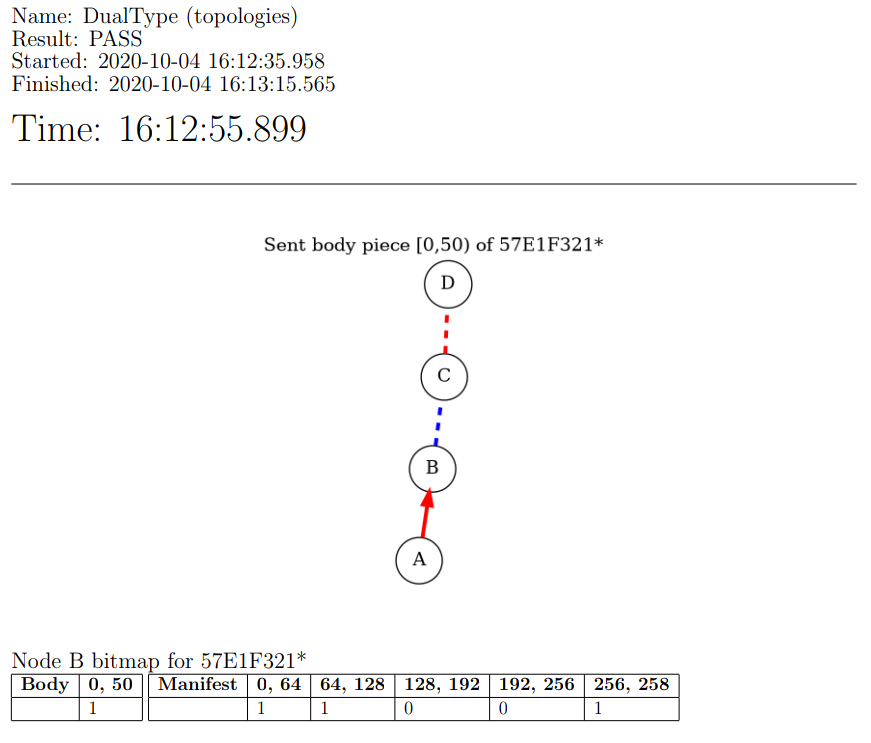
\includegraphics[width=15cm,height=20cm,keepaspectratio]{Figures/Chapter6-PDFPartition.png}
        \caption{PDF Output showing network diagram and bundle bitmap}
        \label{fig:chapter6PDFPartition}
    \end{centering}
\end{figure}

\section{Comparing real-world and framework tests}
The original intentions of this section of the thesis involved the comparison of several tests in the Serval Test Network located at Flinders University, Tonsley Campus with an emulated version of the same network topology.
However, due to the COVID-19 pandemic that occurred during the process of this thesis, this was unable to be conducted due to restrictions around laboratory access.
As such, in this section the reasoning behind why the test network was chosen to be modelled, as well as the criteria that was planned to be used to compare the real-world and framework tests will be detailed and justified for the use of future work.


\subsection{Comparing Tests}
Before tests modelling a real-world scenario could be made, the real-world topology first needed to be determined.
The network that was chosen to be modelled was the Serval Test Network that exists at Flinders University Tonsley.
This network was set up in previous Thesis work and consists of 14 Serval Mesh Extenders \parencite{wade_2019}, with 10 of these Mesh Extenders attached to Serval Mesh Observers that log all WiFi and radio data that the extenders send and receive \parencite{lancaster_2019}.
The lab network was chosen for two main reasons, it allows for comprehensive logging of the functionality of the network due to the Mesh Observers, and the network is set up in a complicated network topology.
The topology of the lab network can be seen in \figurename{ \ref{fig:chapter6LabNetwork}}.

\begin{figure}
    \begin{centering}
        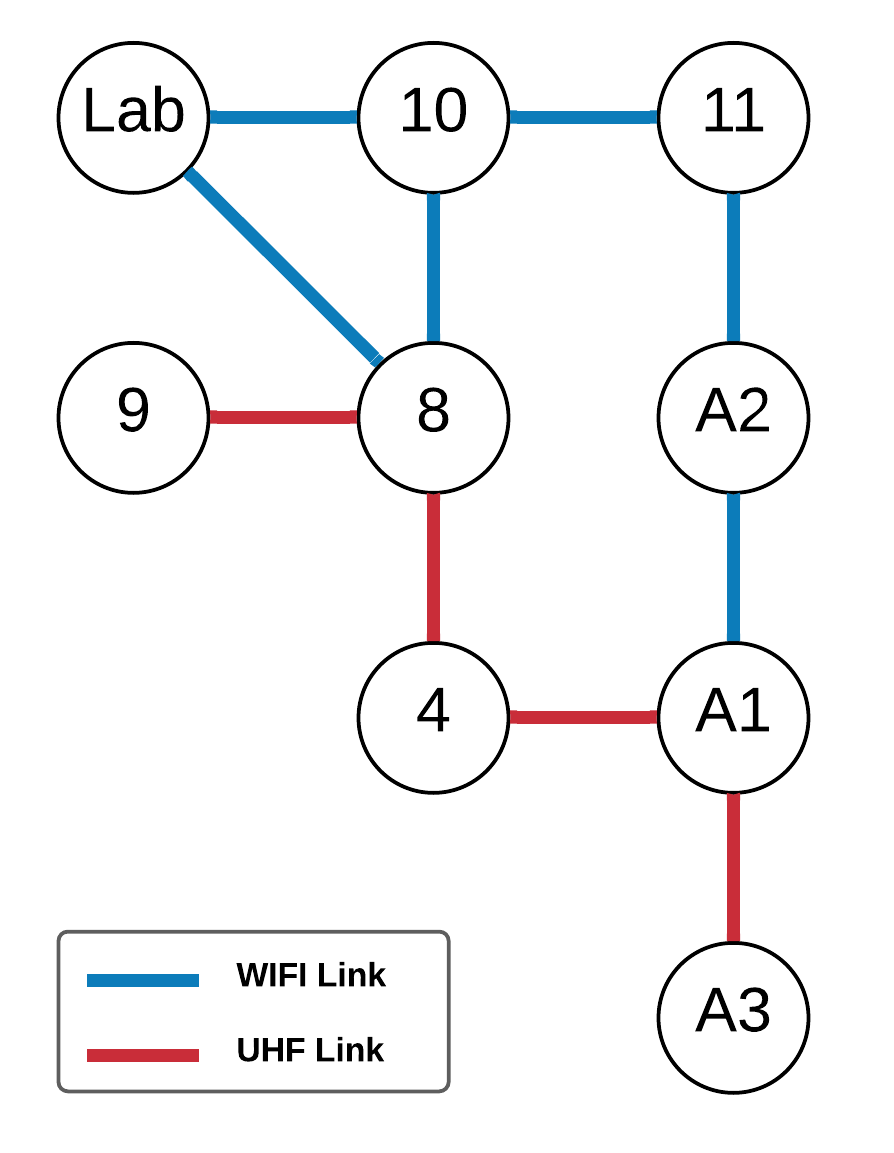
\includegraphics[width=15cm,height=10cm,keepaspectratio]{Figures/Chapter6-LabTopology.png}
        \caption{Network topology of the lab network}
        \label{fig:chapter6LabNetwork}
    \end{centering}
\end{figure}


\subsection{Methodology of comparison}
% What needs to be done
After the network was chosen, several tests were defined to model the Lab Network as outlined in Chapter \ref{Chapter4}.
These tests provide the basis for running tests that model the lab network, and should be expanded to further test aspects of the laboratory network.
Once these tests have been run in the emulation, the existing framework to run tests in the lab network should be used to run these same tests.
After a test has been run in both the test framework and the lab network, the log files of the real-world test should be compiled as outlined earlier in this chapter to form a single comprehensive log file.

% How to compare them
With this, the two networks can then be compared.
Comparison of the real-world and emulated network should be done based on general behaviour and overall functionality rather than comparing for the exact behaviour.
This is due to the fact that individual Serval nodes may make decisions that depend on test-specific information such as sending a bundle earlier than another due to the fact that it was created slightly earlier than the comparable bundle in the other network.

Some behaviour that should be analysed in particular includes:
\begin{itemize}
    \item Multi hop communications
    \item LBARD tree-synchronisation message
    \item LBARD bundle transfers \emph{after} a bundle has already been sent and received
\end{itemize}

The reason this behaviour is of particular note is since each of these behaviours have errors that have been documented to occur in the real-world or in the emulation.
If any of these behaviours are \emph{not} present in one test, but they are in the other, this suggests that the emulation is not accurately modelling the real world, and some investigation must be done to determine what the emulation is lacking.
Similarly, if a fix for a bug like this has been applied, this behaviour should no longer occur in both scenarios as long as the software for both networks has been updated.


% ======== What the advantage of comparing the two is
By comparing the behaviour of the real-world against the behaviour of the emulated Serval network, the simulation fidelity of the software can be determined.
The simulation fidelity is simply how accurately the software is able to model the network, and if it is able to reproduce known real-world problems.
If through analysis the emulation is determined to have a low amount of simulation fidelity, then this indicates to the Serval team that the test framework is not as accurate as believed.
As such, they may need to revisit the test framework and determine how to more accurately model Serval networks.

\section{Summary}
In this chapter, the tools that were developed in Chapter \ref{Chapter5} were adapted to add support for real-world networks.
This involved determining the necessary configurations for LBARD and Serval-DNA processes to produce the necessary log information to allow the tools to monitor when \texttt{LBARD} bundles are sent and received.
As \texttt{fakeradio} can not be used for real-world tests to determine when data is sent by \texttt{LBARD}, this log information is needed to create the major events for diagrams.
Since this log information also contains information about the start and end byte values that LBARD sends, this allowed for the creation of bundle bitmaps, showing a count of the number of times specific pieces of a bundle has been sent to a node.
The bundle bitmaps are displayed as a table in both the ASCII and PDF output types for every LBARD major event, and show a 'live' count of the sent pieces as of the time of that major event.
With this implemented, real-world tests can then be analysed using the tools previously developed in Chapter 5.

% Talk about comparisons
Due to the COVID-19 pandemic, this project was unable to complete the comparison between the emulated and real-world networks due to time constraints. 
The methodology and criteria that is recommended to be used in future investigations into the simulation fidelity of the test framework is outlined. 
This methodology follows the original plan of this thesis and would have been completed if time allowed.

This chapter has continued answering the fourth research question "\fourthRQ" by continuing the development of the diagnostic tools, and has begun answering how these tools might be evaluated.
In the next chapter, this fourth question will conclude being answered, with an in-depth evaluation of the tools developed throughout this thesis.